\documentclass[12pt,a4paper,oneside,brazil]{abntex2}

% Pacotes que serão utilizados%
\usepackage{lmodern}
\usepackage[utf8]{inputenc}
\usepackage[brazil]{babel}
\usepackage[T1]{fontenc}
\usepackage{indentfirst}
\usepackage{graphicx}
\usepackage{microtype}
\usepackage{wrapfig}
\usepackage{multirow}
\usepackage[backend = biber, style=abnt]{biblatex}
\addbibresource{Referencias.bib}

% Informações do documento %
\title{Notas Micro II}
\author{Thiago Oliveira Coelho}
\date{\today}



\begin{document}
\pagestyle{headings}
\pagenumbering{arabic}
\maketitle
\begin{center}
Resumo baseado em \cite{mas}, \cite{nicholson}, \cite{varian} e \cite{pindyck}
\end{center}
\tableofcontents

\chapter{Monopólios}
O monopólio é caracterizado quando há somente uma firma para ofertar para todo o mercado. Neste caso a firma é price-maker. Assim como no competitivo, a firma maximiza seu lucro quando $Cmg = Rmg$, mas nesse caso o $Cmg$ não é igual ao preço, e essa diferença irá nos dar o \emph{grau de Lerner}, que explicita o poder de monopólio da firma:
\[ L = \frac{P - Cmg}{P} = -\frac{1}{\epsilon_{pd}}\]
Esse grau é dado como porcentagem da diferença entre preço e custo marginal. \newline
Outra particularidade é que a receita média neste caso será igual a preço na curva de demanda:
\[ Rme = \frac{RT}{Q} = \frac{P Q}{Q} = P \]
A firma monopolista opera somente na parte da curva aonde a demanda é elástica, pois se esta é inelástica a firma sempre pode voltar na curva de demanda, aumentando o preço e diminuindo seus custos. Podemos também determinar o preço colocado por uma firma monopolista pela seguinte regra:
\[ P = \frac{Cmg}{1 + (\frac{1}{\epsilon_{pd}}}\]

\begin{wrapfigure}{l}{0.5\textwidth}
	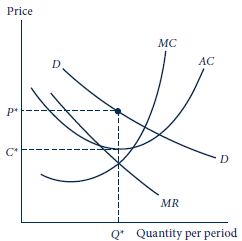
\includegraphics[width=0.4\textwidth]{Monopoly.png}
	\centering
	\caption{Fonte: \cite{nicholson}}
\end{wrapfigure}
O lucro é a diferença entre Preço (Receita média) e o Custo médio. O área do retângulo delimitado por $P^*$ e  $C^*$ representa o lucro do monopolista. A receitar marginal toca o eixo X no ponto em que divide a distância entre 0 e o ponto que a curva de demanda toca o eixo em duas partes iguais; ou seja, a inclinação do CMG é sempre o dobro da incinação da curva de demanda. No longo prazo o monopólio apresentará lucros extraordinários, que representam a remuneração dos fatores que criam o monopólio.
\clearpage

\section{Monopólio com duas plantas}
Neste caso o equilíbrio é dado por:
\[ Cmg_1 = Cmg_2 = Rmg\]
A soma horizontal dos custos marginais resulta no custo marginal total. A quantidade do mercado (Q) é igual a soma das quantidades de cada planta:
\[ Q = Q_1 + Q_2 \]
\begin{figure}[ht]
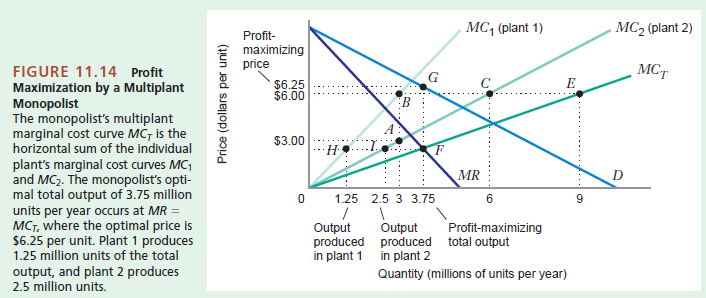
\includegraphics[scale=0.7]{Duas plantas.png}
\centering
\caption{Fonte: \cite{besanko}}
\end{figure}

\section{Custos sociais do monopólio}
O custo social do monopólio equivale ao peso morto criado pelo monopólio quando comparado com a concorrência perfeita. Para observamos as mudanças entre estes dois tipos de organização, iremos comparar os excedentes nas duas situações:

\begin{wrapfigure}{l}{0.5\textwidth}
	\includegraphics[width=0.5\textwidth]{Custo Social do Monopólio.png}
	\centering
	\caption{Fonte: \cite[p. 371]{pindyck}}
\end{wrapfigure}
Como é possível perceber, em monopólio o preço é mais alto e a quantidade menor, excluindo os consumidores na área "B" e "C" do mercado. Essas duas áreas, que numa concorrência perfeita representariam excedente do consumidor, serão peso morto, ou seja, excedente que deixa de existir em organização monopolista. 
\clearpage
Para calcularmos exatamente quanto é o custo social do monopólio usamos:
\[ CS = \frac{(Q_c - Q_m) (P_m - Cmg_m)}{2} \]
Sendo:
\begin{itemize}
\item $Q_c$: Quantidade de equilíbrio em mercado competitivo;
\item $Q_m$: Quantidade de equilíbrio em mercado monopolista;
\item $P_m$: Preço de equilíbrio em mercado monopolista;
\item $Cmg_m$: Custo marginal do monopolista
\end{itemize}

\section{Discriminação}
A discriminação de preços é quando a firma cobra preços diferentes pelo mesmo produto, dependendo de quais forem as características do consumidor. A firma faz isto para poder melhor se apropriar do excedente do consumidor.
\subsection{Discriminação de 1º Grau}
A discriminação de primeiro grau, ou discriminação perfeita, é aquela na qual a firma tem plena capacidade de identificar os consumidores e lhes cobrar preços específicos, e também estes consumidores não conseguem praticar arbitragem.

\begin{wrapfigure}{l}{0.65\textwidth}
	\includegraphics[width=0.65\textwidth]{Discriminação perfeita.png}
	\centering
	\caption{Fonte: \cite[p. 514]{nicholson}}
\end{wrapfigure}

Como é possível perceber, o monopolista consegue cobrar exatamente o preço de reserva de cada consumidor, o que faz este mercado ser eficiente, porém a firma se apropria de todo o excedente do consumidor.
\clearpage
\subsection{Discriminação de 2º Grau}
Numa discriminação de segundo grau a firma irá ter diversos níveis de preço para diferentes quantidades 'caminhando' pela curva de demanda, quanto maior a quantidade menor o preço que pode ser cobrado.
\begin{figure}[h]
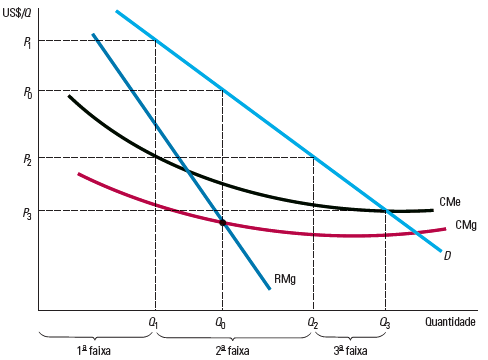
\includegraphics[scale=0.7]{Discriminação segundo grau.png}
\centering
\caption{Fonte : \cite[p. 399]{pindyck}}
\end{figure}
O menor preço cobrado irá coincidir com a curva de custo médio da firma, já que ela não conseguirá cobrar preços menores que aqueles por problemas de custo.

\subsection{Discriminação de 3º Grau}
Na discriminação de terceiro grau a firma se deparará com mais de um mercado que pode ofertar, neste caso teremos dois. Cada um destes mercados possuirá sua curva de demanda específica, e uma curva de demanda total que representa a soma das demandas individuais de cada mercado A decisão econômica de quanto produzir e quanto cobrar em cada mercado será matematicamente similar a decisão de produção da firma em duas plantas. Só que ao invés de haver dois custos marginais e uma receita marginal, há agora duas receitas marginais e um custo marginal somente. A condição de equilíbrio se dá por:
\[ Rmg_1 = Cmg = Rmg_2 \]
A função lucro agora é:
\[ max \pi = Rt_1 + Rt_2 - Ct \]
Pode ser mais sucinto explicitar os preços a serem cobrados nos dois mercados de modo relativo um ao outro. A receita em cada mercado pode ser dada da seguinte forma:
\[ Rmg_i = P_i (1- \frac{1}{\epsilon_{pd}}) \]
Como temos dois mercados, podemos expressar seus preços relativos da seguinte forma:
\[ \frac{P_1}{P_2} = \frac{(1-\frac{1}{\epsilon_{pd2}})}{(1- \frac{1}{\epsilon_{pd1}})} \]
Como seria de se esperar, o maior preço será cobrado daqueles consumidores cuja elasticidade em relação ao produto é menor, portanto podemos estabelecer a seguinte regra:
\begin{itemize}
\item Se $ |\epsilon_{pd1}| > |\epsilon_{pd2}|$ então $ P_1 < P_2$
\item Se $ |\epsilon_{pd1}| < |\epsilon_{pd2}|$ então $ P_1 > P_2$
\end{itemize}
O mercado neste tipo de organização fica deste jeito:
\begin{figure}[h]
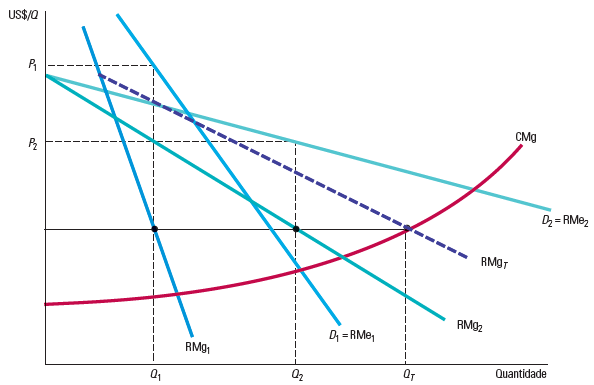
\includegraphics[scale=0.7]{Discriminação terceiro grau.png}
\centering
\caption{Fonte : \cite[p. 402]{pindyck}}
\end{figure}

\section{Impostos e o monopólio}
Definindo um imposto específico de valor $t$ sobre toda unidade de bem produzida, temos que: \newline
Novo Custo: $CT = f(Q) + t Q$ \newline
Novo equilíbrio: $Rmg = Cmg + t$ \newline
Levando em conta uma demanda linear, o ônus do imposto recairá sempre: metade com o consumidor, metade com o produtor. Numa demanda Não linear do tipo:
\[ Q = \frac{K}{P^\alpha} ou Q - k P^\alpha \]
Alfa será sempre a elasticidade preço demanda nesta economia, e a nova regra de determinação de preços será:
\[ P = \frac{Cmg + t}{1 - \frac{1}{\epsilon_p}}\]

\section{Competição monopolística}
É caracterizada pela presença de várias empresas com monopólio sobre suas próprias marcas. Neste caso, o mercado possui vários bens que são substitutos entre si, embora não perfeitos. Cada empresa se defronta com uma curva de demanda negativamente inclinada para seu produto, sendo que esta inclinação é determinada pelo grau de semelhança com os produtos de outras firmas, quanto mais parecidos os produtos, mais plana a curva. Não há restrição para entrada ou saída de firmas, por isso a indústria tem características competitivas. Veja o equilíbrio no curto e longo prazos:

\begin{figure}[h]
	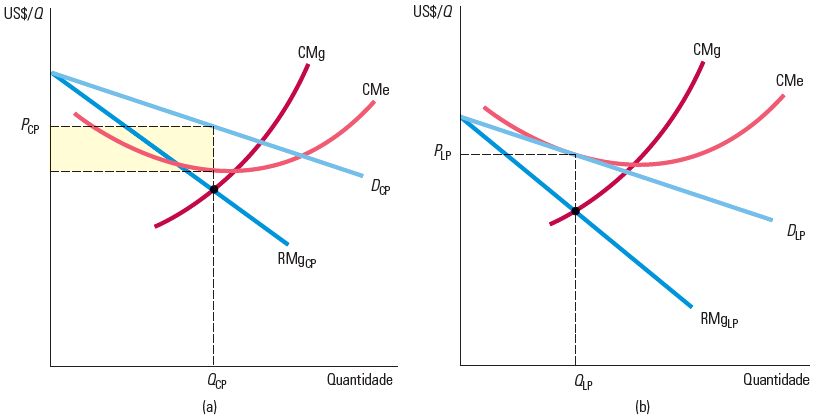
\includegraphics[scale = 0.7]{Competição monopolística.png}
	\centering
	\caption{Fonte: \cite[p. 450]{pindyck}}
\end{figure}

No curto prazo a empresa apresenta lucros anormais ($\pi > 0$), já que no ponto em que seu $Cmg = Rmg$  a curva de demanda está acima do $Cme$. No longo prazo, assim como na competição perfeita, os lucros estimularão a entrada de novos competidores, e nossa firma representativa verá uma queda na demanda pelo seu produto. No equilíbrio de longo prazo $P = Cme$, o que significa que o lucro é normal, já que a área de lucro é representada pela diferença entre $P$ e $Cme$, mas ainda há poder de mercado (mark-up) pois $ P \neq Cmg$. Observe também que comparado com um mercado competitivo, há relativa perda de eficiência, já que a firma não opera no ponto mínimo da curva de custo médio.

\chapter{Oligopólio}
O oligopólio é caracterizado como aquela organização de mercado aonde existem poucas empresas porém mais que uma. Nós iremos nos preocupar em chegar ao equilíbrio de Nash nestes mercados: a situação na qual nenhuma firma tenderá a mudar sua decisão de modo unilateral. Existem diferentes modelos sob os quais podemos analisar este mercado:

\section{Cournot}
No modelo de Cournot as firmas irão responder as mudanças de quantidade uma das outras, por isso temos de desenvolver um modelo de reação de cada firma para depois procurarmos o equilíbrio. Supondo duopólio:

\begin{itemize}
\item Reação da firma 1: $q_1 = f(q_2)$;
\item Reação da firma 2: $q_2 = f(q_1)$.
\end{itemize}

O modelo é caracterizado pelas seguintes hipóteses:
\begin{itemize}
\item Firmas tomam suas decisões simultaneamente; 
\item Bens são homogêneos;
\item Gastos idênticos;
\item Estratégia das firmas não muda;
\item Demanda linear sob a qual as empresas tem pleno conhecimento.
\end{itemize}

Sendo n firmas:
\[ i = 1, 2 , 3, ..., n \Rightarrow Q = q_1 + q_2 + q_3 + ... q_n\]
O equilíbrio de Nash nesse caso é dado por:
\[  \frac{d \pi_i}{d q_i} = \frac{d RT_i}{d q_i} - \frac{d CT_i}{d q_i} = 0\]

\section{Bertrand}
O modelo de Bertrand se dá por duas firmas idênticas, produzindo bens idênticos com custos marginais constantes. A decisão de tais firmas é dada de modo simultâneo,  e o equilíbrio de Nash destas de dá quando seu $P = Cmg$, como se fosse mercado perfeito. A essa conclusão é dado o nome de \emph{paradoxo de Bertrand}, ora, é difícil que a competição entre somente duas firmas seja tão acirrada a ponto de não haver mark-up. Podemos estabelecer as seguintes regras para este mercado (sendo $Q = q_1 + q_2$):
\begin{enumerate}
\item $P_1 > P_2  \Rightarrow q_1 = 0 \Rightarrow$ Firma 1 sai do mercado.
\item $P_1 <  P_2  \Rightarrow  q_1 = Q \Rightarrow$ Firma 2 sai do mercado.
\item $ P_1 = P_2 \Rightarrow q_1 = q_2 = \frac{Q}{2} \Rightarrow$ Firmas repartem o mercado.
\end{enumerate}

\section{Stackelberg}
Este modelo se diferencia por ter decisões sequenciais: uma das firmas (chamada de líder) toma as decisões de produção, e a segunda firma reagirá de acordo com sua função reação, ou seja, a segunda firma age como em um modelo de Cournot. As duas firmas possuem custos idênticos e iguais a zero, além de produto homogêneo. 

\section{Conluio}
Nesse tipo de mercado duas empresas combinam suas produções de tal modo:

\begin{enumerate}
\item Condição de equilíbrio: $ Rmg =Cmg \Rightarrow Q = Q_1 + Q_2 \Rightarrow Q_1 = Q_2 $;
\item Custos fixos idênticos para as duas empresas;
\item Preço é único;
\item Lucro de ambas as empresas é igual;
\end{enumerate}

Comparado aos modelos anteriores o preço é maior, a quantidade menor e lucro das empresas é maior. Podemos fazer uma matriz com as decisões de tais empresas, sendo:
\begin{enumerate}
\item Equilíbrio do modelo de Bertrand;
\item Equilíbrio com conluio.
\end{enumerate}

\begin{table}[h]
\centering
\begin{tabular}{|l|l|l|}
\hline
 & \multicolumn{2}{l|}{Lucro Firma 2} \\ \hline
\multirow{2}{*}{\begin{tabular}[c]{@{}l@{}}Lucro\\ Firma\\ 1\end{tabular}} & 12 , 12 (i) & 20, 4 \\ \cline{2-3} 
 & 4, 20 & 16 , 16 (ii) \\ \hline
\end{tabular}
\end{table}

\section{Liderança de preço ou Mercado com firma dominante}
Nesta organização há uma firma dominante que divide o mercado com diversas firmas satélite. A firma dominante será aquela que define o preço de mercado, por isso possui um mark-up e encontra seu equilíbrio quando $Cmg = Rmg$. As firmas satélite não possuem poder de mercado e portanto estão em equilíbrio quando $Cmg = P$. A demanda do mercado é dada :
\[ D_M = D_D + D_S \]
Demanda do mercado é igual a demanda pela firma dominante mias demanda das firmas satélite.
\begin{figure}[h]
\centering
\includegraphics[scale=0.7]{Firma dominante.png}
\caption{Fonte: \cite[p. 546]{besanko}}
\end{figure}

\section{Cartel} % (fold)
\label{sec:cartel}

O cartel possui as seguintes condições para formação:

\begin{enumerate}
	\item Organização estável;
	\item Espaço para poder de monopólio no mercado.
\end{enumerate}

Sua estrutura típica é:
\begin{enumerate}
	\item Poucas firmas;
	\item Barreiras a entrada;
	\item Produto homogêneo.
\end{enumerate}

São características de sua conduta:

\begin{enumerate}

	\item Incentivos para formação:
	\begin{itemize}
		\item Habilidade de elevação de preços sem induzir a competição de não-membros do cartel;
		\item Poucas punições ao comportamento de cartel;
		\item Baixos custos de organização;
		\item Custo marginal inelástico.
	\end{itemize}

	\item Verificação de conduta dos membros é mais fácil:
	\begin{itemize}
		\item Quanto menos firmas presentes;
		\item Preços não flutuam de modo independente;
		\item Preços são conhecimento de todos;
		\item Membros possuem mesmo ponto de distribuição.
	\end{itemize}

	\item Métodos para prevenir violação:
	\begin{itemize}
	 	\item Fixação de preços;
	 	\item Divisão do mercado por área geográfica ou por clientes;
	 	\item Contratos com clientes.
	\end{itemize} 

	\item Consequências pela violação:
	\begin{itemize}
		\item Guerra de preços;
		\item Fim do cartel.
	\end{itemize}
	\item Desempenho:
	\begin{itemize}
		\item O custo de ineficiência para a sociedade é maior quanto maior a participação de mercado do cartel;
		\item $Q_{cartel} < Q_{comp}$;
		\item Equilíbrio: $Rmg = Cmg$;
		\item Situação análoga ao modelo com firma dominante.
	\end{itemize}

\end{enumerate}
% section cartel (end)
\printbibliography

\section{Teoria dos jogos}
A terminologia que usaremos para abordar teoria dos jogos é a seguinte:

\begin{enumerate}
	\item Jogador: Empresa que participa no jogo;
	\item Jogo: Situação nas quais os jogadores tomam as decisões. Decisões estas que levam em conta as atitudes dos outros jogadores;
	\item Estratégia: Plano que será executado pelo jogador num determinado jogo;
	\item Payoff: Resultado de acordo com a estratégia tomada pelo jogador.
\end{enumerate}

A \emph{estratégia ótima} é aquela que maximiza o payoff de um jogador, presumido racional, num determinado jogo. Uma \emph{estratégia dominante} é aquela que é ótima independentemente do que o oponente venha a fazer. Os jogos podem ser tanto cooperativos quanto não cooperativos.Enquanto num jogo cooperativo é possível haver formação de contrato entre os jogadores, isso é impossível em jogos não cooperativos.

\end{document}
